\documentclass[11pt]{article}
\usepackage[margin=1in]{geometry}
\usepackage{amsmath,booktabs,graphicx,hyperref}
\hypersetup{colorlinks=true,urlcolor=blue}
\title{Prescribed-front Icepack experiment at EKaS:\\implementation, synthetic results and remaining problems}
\author{Icepack-Sediment}
\date{8 October 2026}
\begin{document}
\maketitle
\noindent\textbf{Result status.} Both synthetic experiments completed a common
25-year spinup and the 1953--2021 transient in Firedrake/UW Icepack. At the
comparison gate, the advancing case is 67.83 m thicker and 515.54 m/year slower
than the fixed-front control in 2021. These results validate a numerical
experiment; they are not EKaS predictions or agreement with the publication.
A regional run could not start because prepared regional inputs are missing.
A geometry audit also rejects the tested straight corridor.

The repository is public. The exact \texttt{AGENTS.md} and academic style guide
were copied from OMP-OOI main. OMP-OOI has no standalone plotting style file;
the implementation reuses the rcParams block from its energy-likelihood analysis
and 220 dpi exports. Source commits and hashes are recorded in
\texttt{template\_provenance.json}. All implementation changes remain on the
feature branch in pull request 1.

\section{Relationship to Figure 13}
Dachauer et al. (2026), doi:\href{https://doi.org/10.1017/jog.2026.10172}{10.1017/jog.2026.10172},
Figure 13, compares prescribed front advance with a fixed-front control.
The gate here lies 1 km upstream of the nominal 1953 front. The paper initializes
from 2021 geometry, inverts fluidity and slipperiness, relaxes for two years,
re-inverts, truncates at the 1953 front and relaxes for 25 years. This code
implements truncation, common relaxation and paired transients, but not the
inversions. It does not reconstruct a measured 1953 surface.
The front offsets are 0, 960, 1400 and 1820 m at 1953, 1985, 2007 and 2021.
They integrate rounded published advance rates rather than mapped front lines.
Editable CSV observations drive monotone PCHIP; piecewise-linear interpolation
is available to follow the paper's interpolation convention.

\begin{figure}[ht]
\centering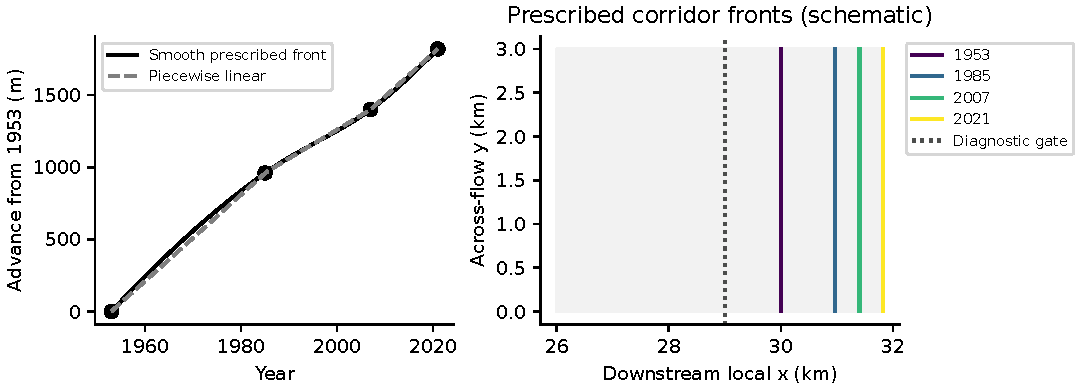
\includegraphics[width=\linewidth]{../results/figures/prescribed_terminus.pdf}
\caption{Approximate prescribed chronology and schematic model front positions.
The lines are not mapped historical terminus boundaries.}
\end{figure}

\section{Physics and moving domain}
Icepack \texttt{IceStream} supplies SSA dynamics, Glen exponent 3, ocean
traction and hydrostatic grounded/floating surface geometry. Regional forcing
is intended to use a fixed MAR 2021 SMB field and observed upstream velocity
and thickness. Those fields have not yet been prepared. Synthetic tests use
zero SMB, a sloping synthetic bed and surface, and prescribed inflow.
With speed $v$, $k=C_{\rm Ua}^{-1/3}$ and effective pressure $N$, sliding follows
\[
 t_b=\frac{\mu N k v^{1/3}}{\mu N+k v^{1/3}},\qquad
 N=\max\{\rho_i gH-\rho_w g\max(-z_b,0),0\},\quad z_b=s-H.
\]
Floating ice has zero basal traction. A 16-point speed quadrature integrates the
traction to obtain Icepack's dissipation potential; speed is regularized at
0.001 m/year. The default $\mu=0.5$, uniform fluidity $A=10$ in MPa--m--year
units and supplied/prior friction are assumptions, not recovered Ua parameters.
Side walls allow tangential sliding with configurable drag.

Each timestep builds an identically ordered triangular corridor mesh at the
prescribed length. Thickness transfer uses the old/new length ratio to preserve
volume; implicit continuity uses physical velocity minus mesh velocity. This
first-order ALE split creates no arbitrary new ice slab and records discharge
relative to the moving boundary. It is a straight constant-width domain, not
the curved glacier catchment. CG1 sampling uses actual triangle connectivity.
Serial execution is required. Negative or nonfinite thickness aborts rather
than being clipped. Fresh meshes and form construction make long runs expensive.

\section{Executed simulations and checks}
The local Docker image \texttt{vdv-ice-shelf} supplies working Firedrake and
UW Icepack. The full synthetic pair used a 12 by 4 mesh, $\Delta t=0.25$ year,
25-year spinup and 68-year transient. The retained production potential uses
16-point speed quadrature and Icepack's spatial degree 2 for CG1 spaces.

\begin{table}[ht]\centering
\begin{tabular}{lrr}\toprule
Quantity & Fixed & Advancing\\\midrule
Minimum thickness over run (m) & 431.82 & 408.40\\
Maximum relative mass residual & $3.91\times10^{-16}$ & $4.50\times10^{-16}$\\
2021 front offset (m) & 0 & 1820\\
2021 gate thickness (m) & 482.57 & 550.41\\
2021 gate speed (m/year) & 3173.47 & 2657.93\\
2021 gate flux (Gt/year) & 4.21292 & 4.02450\\\bottomrule
\end{tabular}
\caption{Actual full-duration synthetic outputs. Mass residual is the continuity
volume error divided by volume; closure alone does not establish positivity or accuracy.}
\end{table}

The validator passed identical input/configuration and initial-state hashes,
equal post-spinup fields, stationary control front, prescribed advancing front,
positive thickness, mass balance and the expected qualitative slowdown/thickening.
Advancing-minus-control flux is $-0.18842$ Gt/year. Five unit tests passed for
chronology, friction limits and raster preprocessing (grounded/floating thickness,
SMB units, velocity rotation and nodata rejection). Firedrake checks passed CG1
sampling, conservative transfer and 16 traction-derivative cases.
The executed notebook retains outputs and imports the core implementation.

An experimental analytic potential also completed the full pair: final gate
thickening was 67.8368 m and slowdown 515.5849 m/year. Short tests with spatial
degrees 12 and 24 differed by less than $5\times10^{-13}$ in gate speed/flux.
The analytic variant was not retained: no controlled runtime benefit was
established. Its recorded results describe that experiment, not an additional
production mode. Neither these checks nor mass closure establish mesh or
timestep convergence.

\begin{figure}[p]\centering
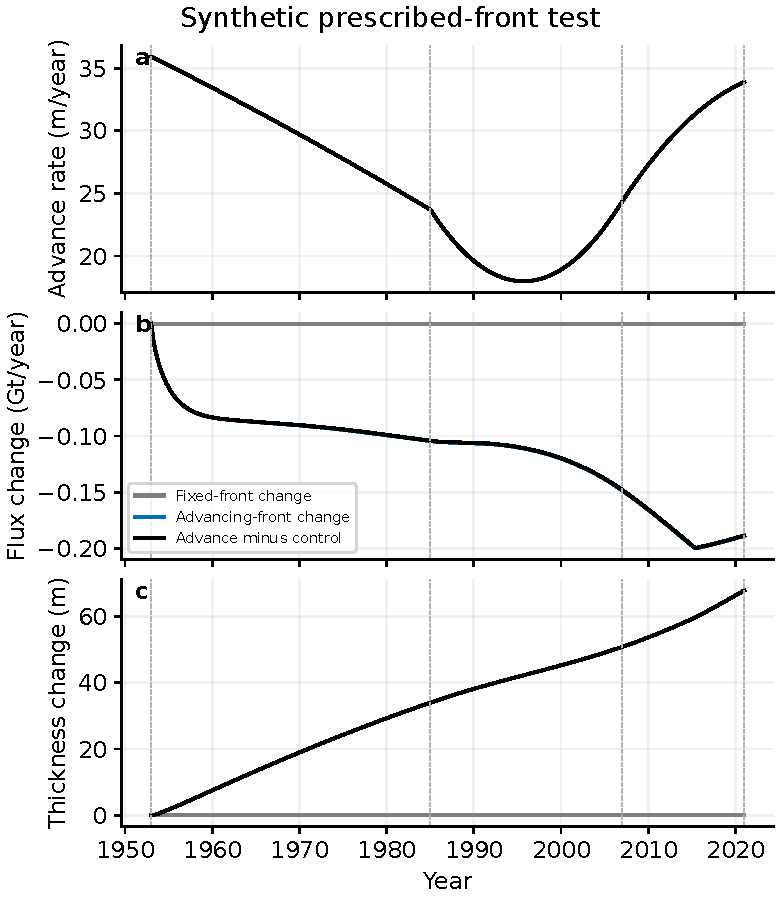
\includegraphics[width=\linewidth]{figures/synthetic_full/figure13_comparison.pdf}
\caption{Executed synthetic gate comparison. The data and magnitudes are not calibrated EKaS results.}
\end{figure}

\begin{figure}[p]\centering
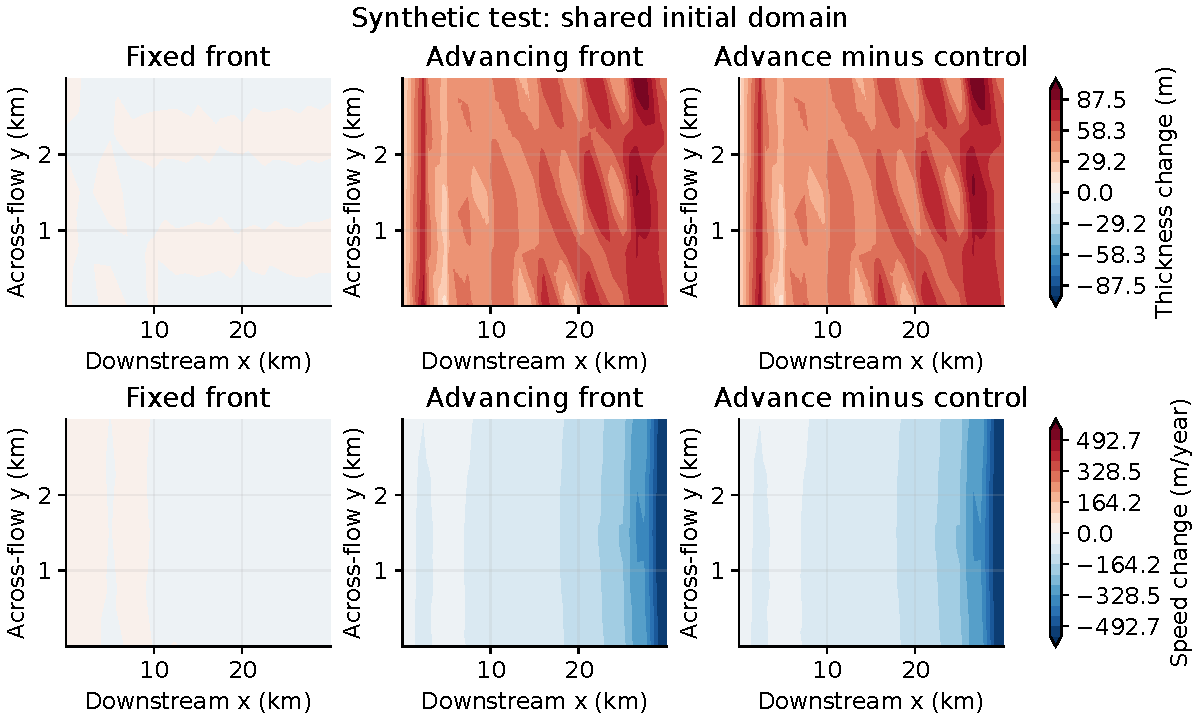
\includegraphics[width=\linewidth]{figures/synthetic_full/spatial_comparison.pdf}
\caption{Synthetic spatial changes relative to the common post-spinup state and advancing-minus-control differences on the initial domain.}
\end{figure}

\section{Problems found}
A one-year timestep failed during the common spinup at elapsed year 4 with
negative thickness, before any advancing-front forcing. Both the original and
experimental analytic potential showed this failure; the latest saved analytic
failure had minimum thickness $-7535.07$ m. Partial histories and failure JSON
are retained locally. The quarter-year pair stayed positive, but halving that
timestep and refining the mesh remain necessary. CG1 transport and split
stress/continuity updates do not guarantee positivity.

Cached BedMachine Greenland v6 and a modern flowline enabled a geometry probe.
The candidate 30 km by 3 km straight corridor used the modern front minus a
2 km fjord extension and the approximate 1820 m advance to estimate the initial
front. Of sampled initial grid points, 25.94\% fell outside the ice mask and
23.19\% had nonpositive thickness. These are sampled-point fractions, not exact
area fractions. The candidate cannot be used as positive-thickness regional
input. This audit does not rule out every alternative corridor; a curved
ice-conforming domain or a verified narrower trunk is needed.

\begin{figure}[ht]\centering
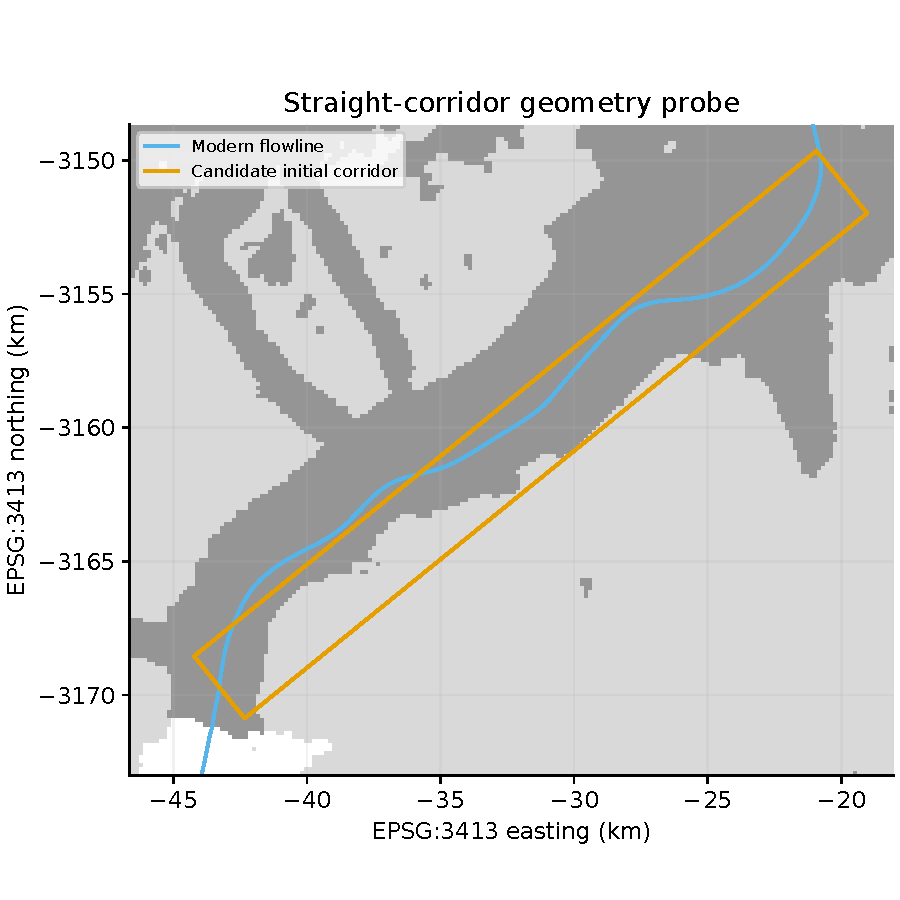
\includegraphics[width=\linewidth]{figures/candidate_corridor.pdf}
\caption{Geometry probe using cached BedMachine v6 and a modern flowline.
The candidate initial front is approximate, not a surveyed 1953 boundary.}
\end{figure}

The regional invocation failed with missing \texttt{data/processed/ekas.npz}.
Cached summer-2023 MEaSUREs velocities cannot silently replace annual-2021
velocity. MAR 2021 SMB, verified historical boundaries, calibrated friction and
fluidity and the author's corrected/kriged bed remain unavailable to this run.
BedMachine v6 is an available substitute, not the paper's exact corrected bed.
The plotting environment lacks Rasterio; all five preprocessing tests instead
passed in the separate \texttt{ekas-figure} environment. Default Python lacks
Firedrake/Icepack; the Docker checks establish availability only in that image.

\section{Reproduction and next work}
The README documents installation, input preparation, paired runs, validation,
figure generation and report compilation. Raw regional data and simulation
archives are ignored by git. Source information and units are documented in
\texttt{data/README.md}; small plots and validation summaries are committed.
The figure script rejects incomplete simulations and explicitly labels synthetic
results. Historical panels remain unavailable rather than being filled with
invented model output.

Prepare valid regional geometry and 2021 forcing/velocity, calibrate the stress
balance, replace rounded offsets with mapped boundaries and assess the corrected
bed before interpreting the Figure 13 comparison. Then check spatial/temporal
convergence and compare flux, velocity and dynamic thickening. Main differences
from Ua include the trunk boundary conditions, missing inversion/re-inversion,
uniform fluidity, approximate fronts, stock bed and first-order corridor ALE
transport. Their influence on quantitative agreement remains unresolved.
Explicit sediment thickness and bank geometry are the planned next step after
the geometric experiment is established.
\end{document}
